% This LaTeX document needs to be compiled with XeLaTeX.
\documentclass[10pt]{article}
\usepackage[utf8]{inputenc}
\usepackage{graphicx}
\usepackage[export]{adjustbox}
\graphicspath{ {./images/} }
\usepackage{amsmath}
\usepackage{amsfonts}
\usepackage{amssymb}
\usepackage[version=4]{mhchem}
\usepackage{stmaryrd}
\usepackage{multirow}
\usepackage[fallback]{xeCJK}
\usepackage{polyglossia}
\usepackage{fontspec}
\setCJKmainfont{Noto Serif CJK TC}

\setmainlanguage{polish}
\setmainfont{CMU Serif}

\title{KOD }

\author{}
\date{}


\newcommand\Varangle{\mathop{{<\!\!\!\!\!\text{\small)}}\:}\nolimits}

\begin{document}
\maketitle
\section*{PESEL}
\begin{center}

\includegraphics[max width=\textwidth]{2024_11_21_832f1bc2b626663f1df2g-01(1)}
\end{center}

WEOCEAWEK\\
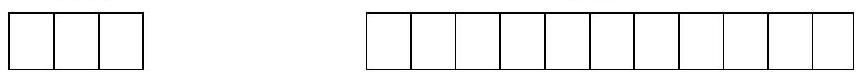
\includegraphics[max width=\textwidth, center]{2024_11_21_832f1bc2b626663f1df2g-01}

\section*{PRÓBNY EGZAMIN MATURALNY Z MATEMATYKI}
\section*{POZIOM PODSTAWOWY}
\begin{enumerate}
  \item Sprawdź, czy arkusz egzaminacyjny zawiera 18 stron (zadania 1-34). Ewentualny brak zgłoś przewodniczącemu zespołu nadzorującego próbny egzamin.
  \item Rozwiązania zadań i odpowiedzi wpisuj w miejscu na to przeznaczonym.
  \item Odpowiedzi do zadań zamkniętych (1-25) przenieś na kartę odpowiedzi, zaznaczając je w części karty przeznaczonej dla zdającego. Zamaluj - pola do tego przeznaczone. Błędne zaznaczenie otocz kółkiem i zaznacz właściwe.
  \item Pamiętaj, że pominięcie argumentacji lub istotnych obliczeń
\end{enumerate}

Marzec 2019

Czas pracy:\\
170 minut

Liczba punktów do uzyskania: 50\\
w rozwiązaniu zadania otwartego (26-34) może spowodować, że za to rozwiązanie nie będziesz mógł dostać pełnej liczby punktów.\\
5. Pisz czytelnie i używaj tylko długopisu lub pióra z czarnym tuszem lub atramentem.\\
6. Nie używaj korektora, a błędne zapisy wyraźnie przekreśl.\\
7. Pamiętaj, że zapisy w brudnopisie nie będą oceniane.\\
8. Możesz korzystać z zestawu wzorów matematycznych, cyrkla i linijki oraz kalkulatora.\\
9. Na karcie odpowiedzi wpisz swój numer PESEL.\\
10. Nie wpisuj żadnych znaków w części przeznaczonej dla egzaminatora.

\section*{ZADANIA ZAMKNIĘTE}
W zadaniach od 1. do 25. wybierz i zaznacz na karcie odpowiedzi poprawna odpowiedź. Zadanie 1. (0-1 pkt)\\
Wśród liczb \(a, b, c, d\) liczbą całkowitą jest\\
A. \(a=\frac{2^{5} \cdot 27^{\frac{2}{3}}}{4^{9}}\)\\
B. \(b=\frac{8^{4} \cdot 2}{3^{2}}\)\\
C. \(c=\frac{3^{5} \cdot 8^{\frac{4}{3}}}{36^{\frac{1}{2}}}\)\\
D. \(d=\frac{2^{0}}{2^{2} \cdot 8}\)

\section*{Zadanie 2. (0-1 pkt)}
Jeżeli \(a=\log _{2}(5 \sqrt[3]{2})-\log _{2} 5 \quad\) i \(\quad b=\log _{3} 15+\log _{3} \frac{\sqrt{3}}{45}\), to wartość wyrażenia \(a^{b}\) jest równa\\
A. \(\sqrt{2}\)\\
B. \(\sqrt{3}\)\\
C. 9\\
D. \(\sqrt[3]{2}\)

\section*{Zadanie 3. (0-1 pkt)}
Oszacowano, że do malowania pokoju potrzeba 17 litrów farby. W rzeczywistości zużyto 20 litrów. Błąd względny szacowania wyrażony w procentach wynosi\\
A. \(0,15 \%\)\\
B. \(15 \%\)\\
C. \(17,6 \%\)\\
D. \(85 \%\)

\section*{Zadanie 4. (0-1 pkt)}
Cenę towaru dwukrotnie obniżano o \(20 \%\). W wyniku obniżek cena towaru wynosi 96 zł. Przed zmianami towar kosztował\\
A. \(138,24 \mathrm{zł}\)\\
B. \(144,00 \mathrm{zł}\)\\
C. \(150,00 \mathrm{zł}\)\\
D . 160,00 zł

\section*{Zadanie 5. (0-1 pkt)}
Funkcja \(f(x)=\frac{6 x-x^{2}}{x^{2}-36}\)\\
A. ma jedno miejsce zerowe \(x=0\)\\
B. ma dwa miejsce zerowe \(x=0, x=6\)\\
C. ma dwa miejsce zerowe \(x=6, x=-6\)\\
D. ma trzy miejsce zerowe \(x=0, x=6, x=-6\)

Zadanie 6. (0-1 pkt)\\
Na rysunku przedstawiono wykres funkcji określonej wzorem\\
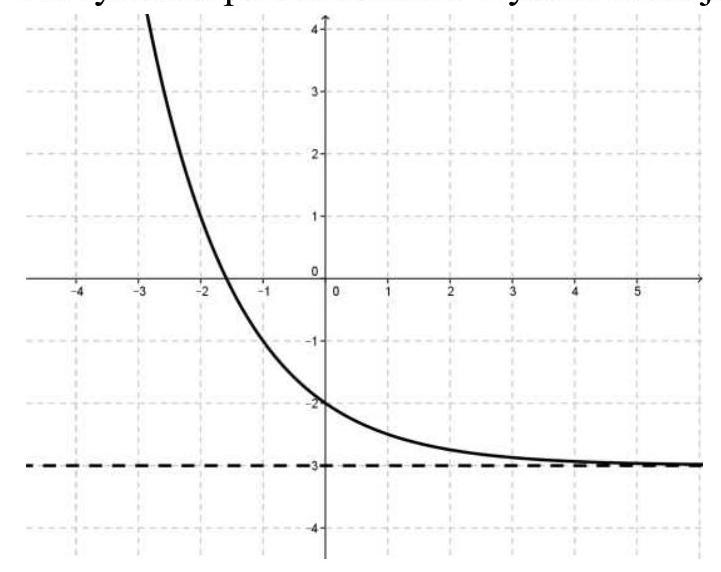
\includegraphics[max width=\textwidth, center]{2024_11_21_832f1bc2b626663f1df2g-02}\\
A. \(f(x)=2^{x}-3\)\\
B. \(f(x)=2^{x-3}\)\\
C. \(f(x)=\left(\frac{1}{2}\right)^{x}-3\)\\
D. \(f(x)=\left(\frac{1}{2}\right)^{x-3}\)

\section*{BRUDNOPIS}
\begin{center}

\includegraphics[max width=\textwidth]{2024_11_21_832f1bc2b626663f1df2g-03}
\end{center}

\section*{Zadanie 7. (0-1 pkt)}
Wartość funkcji \(f(x)=\frac{-x^{2}-2 x}{x-2}\) dla argumentu równego \(-2+\sqrt{2}\) wynosi\\
A. -1\\
B. \(\sqrt{2}-2\)\\
C. \(\frac{\sqrt{2}-10}{7}\)\\
D. \(\frac{-3 \sqrt{2}+2}{7}\)

\section*{Zadanie 8. (0-1 pkt)}
Wykres funkcji liniowej \(f(x)=a x+b \quad\) dla \(a<0\) i \(b>0 \quad\) przechodzi przez ćwiartki układu współrzędnych\\
A. \(I, I I, I V\)\\
B. I, III, IV\\
C. I,II,III\\
D. II,III,IV

\section*{Zadanie 9. (0-1 pkt)}
Maksymalnym przedziałem w którym funkcja kwadratowa \(f(x)=-3(x+2)^{2}-7\) jest malejąca jest zbiór\\
A. \(\langle 2,+\infty)\)\\
B. \((-\infty, 2)\)\\
C. \((-2,+\infty)\)\\
D. \((-\infty,-2\rangle\)

\section*{Zadanie 10. (0-1 pkt)}
Dany jest ciąg \(\left(a_{n}\right)\) określony wzorem ogólnym \(a_{n}=3^{n}-3^{2}\). Wyraz \(a_{n+2}\) tego ciągu dla \(n=3\) jest równy\\
A. 3\\
B. 18\\
C. 27\\
D. 234

\section*{Zadanie 11. (0-1 pkt)}
Pierwszy wyraz ciągu arytmetycznego wynosi 7, suma siedmiu początkowych wyrazów ciągu jest równa (-14). Czwarty wyraz ciągu jest równy\\
A. -11\\
B. -3\\
C. -2\\
D. 16

\section*{Zadanie 12. (0-1 pkt)}
Za wykopanie pierwszego metra studni zapłacono 75 złotych. Wykopanie każdego następnego metra kosztowało dwa razy tyle co poprzedniego. Za wykopanie studni zapłacono 76725 złotych. Głębokość studni wynosiła\\
A. \(7 m\)\\
B. \(8 m\)\\
C. 9 m\\
D. 10 m

\section*{Zadanie 13. (0-1 pkt)}
Ramię końcowe kąta \(\alpha \in\left(90^{\circ} ; 180^{\circ}\right)\) zawiera się w prostej \(y=-\frac{3}{4} x\). Zatem\\
A. \(\sin \alpha=-\frac{3}{4}\)\\
B. \(\sin \alpha=-\frac{3}{5}\)\\
C. \(\sin \alpha=\frac{3}{5}\)\\
D. \(\sin \alpha=\frac{4}{5}\)

\section*{BRUDNOPIS}
\begin{center}

\includegraphics[max width=\textwidth]{2024_11_21_832f1bc2b626663f1df2g-05}
\end{center}

\section*{Zadanie 14. (0-1 pkt)}
Kąt \(\alpha\) jest kątem ostrym i \(\cos \alpha=\frac{\sqrt{3}}{3}\). Zatem\\
A. \(\alpha=30^{\circ}\)\\
B. \(\alpha \in\left(30^{\circ}, 45^{\circ}\right)\)\\
C. \(\alpha \in\left(45^{\circ}, 60^{\circ}\right)\)\\
D. \(\alpha=60^{\circ}\)

\section*{Zadanie 15. (0-1 pkt)}
Dla ostrego kąta \(\alpha\) wyrażenie \(\cos \alpha \cdot \frac{\operatorname{tg} \alpha}{\sin \alpha}\) jest równe\\
A. \(\frac{\sin \alpha}{\cos \alpha}\)\\
B. \(\frac{\sin ^{2} \alpha}{\cos ^{2} \alpha}\)\\
C. \(\frac{\cos ^{2} \alpha}{\sin ^{2} \alpha}\)\\
D. \(\sin ^{2} \alpha+\cos ^{2} \alpha\)

\section*{Zadanie 16. (0-1 pkt)}
Punkty \(A, B, C\) leżą na okręgu o środku \(S\) (rysunek), \(|\Varangle \mathrm{ASC}|=150^{\circ}\) oraz \(|\Varangle \mathrm{ACB}|=42^{\circ}\). Miara kąta \(B A C\) jest równa\\
A. \(15^{\circ}\)\\
B. \(42^{\circ}\)\\
C. \(52,5^{\circ}\)\\
D. \(63^{\circ}\)\\
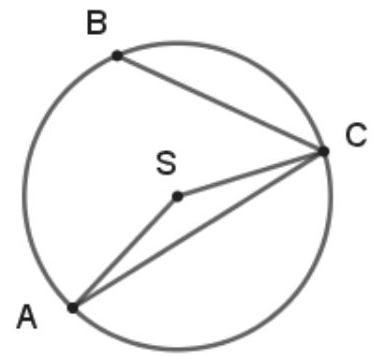
\includegraphics[max width=\textwidth, center]{2024_11_21_832f1bc2b626663f1df2g-06}

\section*{Zadanie 17. (0-1 pkt)}
Punkty A, B, C są punktami przecięcia paraboli o równaniu \(y=-x^{2}+2 x+8 \mathrm{z}\) osiami układu współrzędnych. Pole trójkąta \(A B C\) jest równe\\
A. 8\\
B. 9\\
C. 24\\
D. 27

\section*{Zadanie 18. (0-1 pkt)}
Dane są okręgi styczne wewnętrznie o środkach \(A\) i \(B\). Wiadomo, że promień jednego okręgu jest trzy razy dłuższy od promienia drugiego okręgu i \(|A B|=2 \frac{2}{3}\). Promienie tych okręgów mają długość\\
A. \(\frac{1}{3} i 3\)\\
B. \(1 \frac{1}{2} i 4 \frac{1}{2}\)\\
C. \(\frac{2}{3} i 2\)\\
D. \(1 \frac{1}{3} i 4\)

\section*{Zadanie 19. (0-1 pkt)}
Proste o równaniach \(k: y=(3-2 m) x+10\) i \(l: y=\frac{3}{1-6 m} x-2 m\) są prostopadłe dla\\
A. \(m=\frac{5}{6}\)\\
B. \(m=\frac{6}{5}\)\\
C. \(m=-\frac{5}{3}\)\\
D. \(m=\frac{5}{3}\)

\section*{Zadanie 20. (0-1 pkt)}
Punkty \(A=(-2 ; 3), B=(1 ;-4), C=(3 ; 4)\) są kolejnymi wierzchołkami równoległoboku \(A B C D\). Równanie prostej zawierającej bok \(A D\) tego równoległoboku ma postać\\
A. \(-4 x+y-11=0\)\\
B. \(4 x+y+11=0\)\\
C. \(-4 x-y+3=0\)\\
D. \(4 x-y+3=0\)

\section*{BRUDNOPIS}
\begin{center}

\includegraphics[max width=\textwidth]{2024_11_21_832f1bc2b626663f1df2g-07}
\end{center}

\section*{Zadanie 21. (0-1 pkt)}
Dany jest odcinek AB , gdzie \(A(-4,16), B(-8,10)\). Punkt \(S\) jest środkiem odcinka \(A B\).\\
Obrazem punktu \(S\) w symetrii względem osi \(O Y\) jest punkt\\
A. \(S^{\prime}(-6,13)\)\\
B. \(S^{\prime}(6,13)\)\\
C. \(S^{\prime}(-6,-13)\)\\
D. \(S^{\prime}(6,-13)\)

\section*{Zadanie 22. (0-1 pkt)}
Przekrój osiowy stożka jest trójkątem równoramiennym o ramieniu długości 12. Kąt rozwarcia stożka ma miarę \(120^{\circ}\). Objętość stożka wynosi\\
A. \(72 \pi\)\\
B. \(72 \sqrt{3} \pi\)\\
C. \(216 \pi\)\\
D. \(216 \sqrt{3} \pi\)

\section*{Zadanie 23. (0-1 pkt)}
Przekątne dzielą równoległobok na cztery trójkąty\\
A. przystające\\
B. podobne\\
C. o równych polach\\
D. o równych obwodach

\section*{Zadanie 24. (0-1 pkt)}
Ze zbioru \(\{1,2,3,4,5,6,7,8,9,10,11\}\) losujemy bez zwracania dwa razy po jednej liczbie. Wylosowane liczby tworzą parę \((x, y)\), gdzie \(x\) jest pierwszą wylosowaną liczbą, \(y\) jest drugą wylosowaną liczbą. Wszystkich par \((x, y)\) takich, że suma \(x+y\) jest liczbą parzystą jest\\
A. 20\\
B. 25\\
C. 50\\
D. 61

\section*{Zadanie 25. (0-1 pkt)}
Wojtek notował temperaturę powietrza o godzinie 12.00 w pięciu kolejnych dniach stycznia.\\
Otrzymał następujące wyniki:

\begin{center}
\begin{tabular}{|l|c|c|c|c|c|}
\hline
Data & 15.01 & 16.01 & 17.01 & 18.01 & 19.01 \\
\hline
Temperatura & 3 & 2 & -2 & -5 & -3 \\
\hline
\end{tabular}
\end{center}

Odchylenie standardowe od średniej temperatury w tych dniach, z dokładnością do 0,1 wynosi\\
A. 1,0\\
B. 3,0\\
C. 3,6\\
D. 9,2

\section*{BRUDNOPIS}
\begin{center}

\includegraphics[max width=\textwidth]{2024_11_21_832f1bc2b626663f1df2g-09}
\end{center}

\section*{ZADANIA OTWARTE}
Rozwiazania zadań o numerach od 26. do 34. nalė̇y zapisać w wyznaczonych miejscach pod treścia zadania.

\section*{Zadanie 26. (0-2 pkt)}
Na rysunku przedstawiony jest wykres funkcji \(y=f(x)\). Podaj zbiór wartości funkcji \(g(x)=f(x+1)-2\).\\
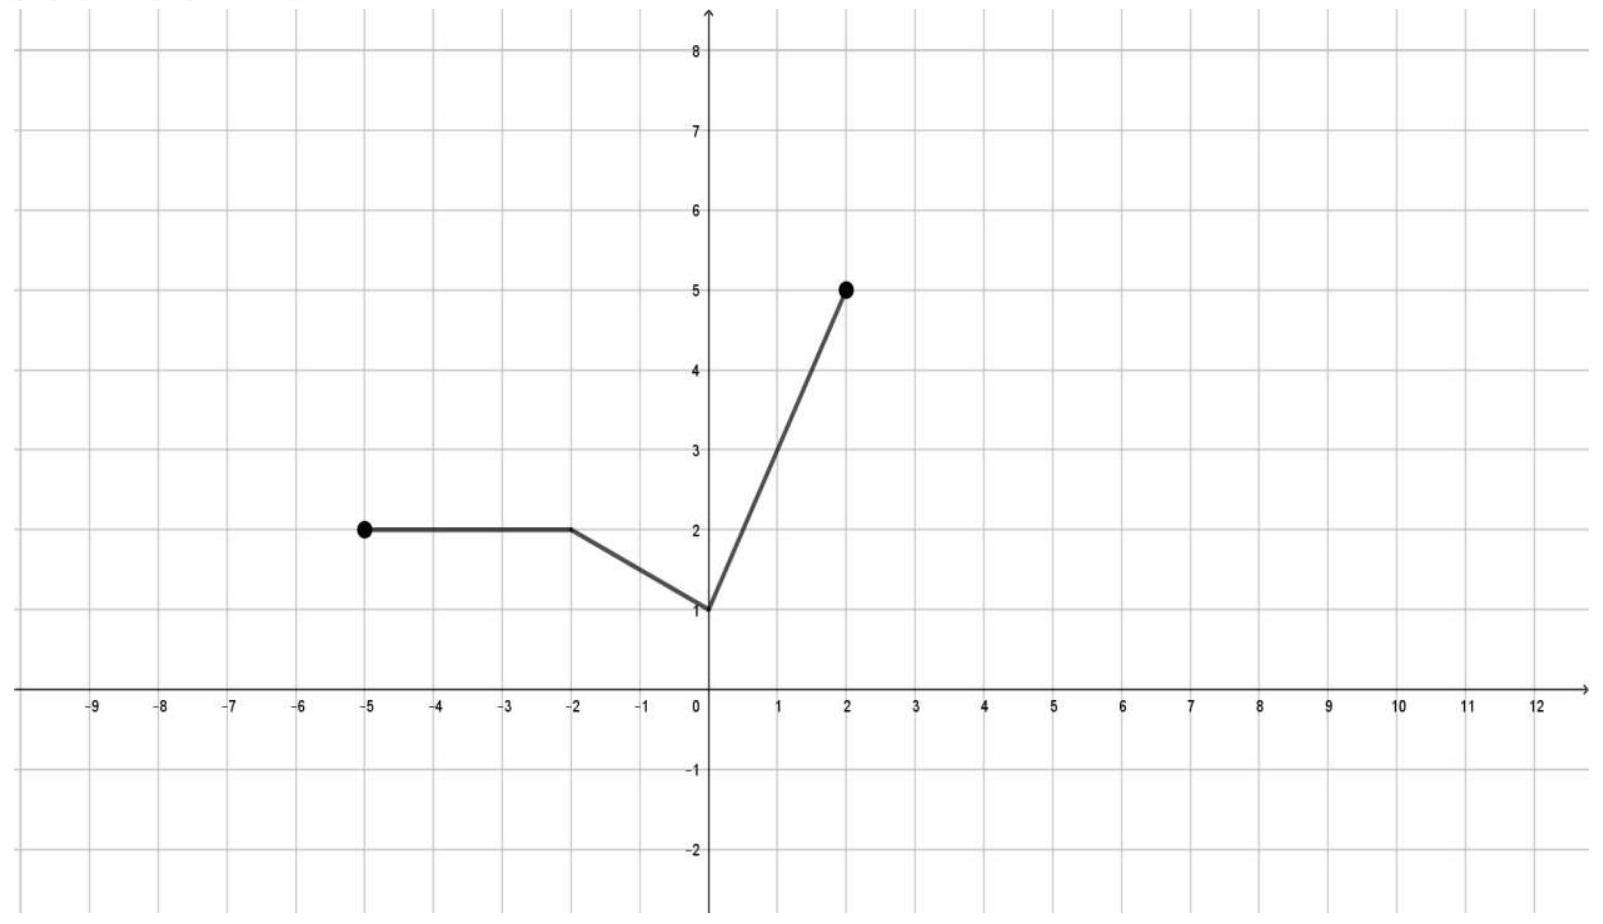
\includegraphics[max width=\textwidth, center]{2024_11_21_832f1bc2b626663f1df2g-10(1)}\\

\includegraphics[max width=\textwidth, center]{2024_11_21_832f1bc2b626663f1df2g-10}

Odpowiedź:

\section*{Zadanie 27. (0-2 pkt)}
Rozwiąż nierówność: \(-\frac{1}{2} x(x+2)<1\).\\

\includegraphics[max width=\textwidth, center]{2024_11_21_832f1bc2b626663f1df2g-11(4)}

Odpowiedź:

\section*{Zadanie 28. (0-2 pkt)}
Udowodnij, że reszta z dzielenia sumy kwadratów dwóch kolejnych liczb naturalnych niepodzielnych przez 3, przy dzieleniu przez 18 jest równa 5.

\begin{center}
\begin{tabular}{|c|c|c|c|c|c|c|c|c|c|c|c|c|c|c|c|c|c|c|c|c|c|c|c|c|c|c|c|c|}
\hline
 &  &  &  &  &  &  &  &  &  &  &  &  &  &  &  &  &  &  &  &  &  &  &  &  &  &  &  &  \\
\hline
 &  &  &  &  &  &  &  &  &  &  &  &  &  &  &  &  &  &  &  &  &  &  &  &  &  &  &  &  \\
\hline
 &  &  &  &  &  &  &  &  &  &  &  &  &  &  &  &  &  &  &  &  &  &  &  &  &  &  &  &  \\
\hline
 &  &  &  &  &  &  &  &  &  &  &  &  &  &  &  &  &  &  &  &  &  &  &  &  &  &  &  &  \\
\hline
 &  &  &  &  &  &  &  &  &  &  &  &  &  &  &  &  &  &  &  &  &  &  &  &  &  &  &  &  \\
\hline
 &  &  &  &  &  &  &  &  &  &  &  &  &  &  &  &  &  &  &  &  &  &  &  &  &  &  &  &  \\
\hline
 &  &  &  &  &  &  &  &  &  &  &  &  &  &  &  &  &  &  &  &  &  &  &  &  &  &  &  &  \\
\hline
 &  &  &  &  &  &  &  &  &  &  &  &  &  &  &  &  &  &  &  &  &  &  &  &  &  &  &  &  \\
\hline
 &  &  &  &  &  &  &  &  &  &  &  &  &  &  &  &  &  &  &  &  &  &  &  &  &  &  &  &  \\
\hline
 &  &  &  &  &  &  &  &  &  &  &  &  &  &  &  &  &  &  &  &  &  &  &  &  &  &  &  &  \\
\hline
 &  &  &  &  &  &  &  &  &  &  &  &  &  &  &  &  &  &  &  &  &  &  &  &  &  &  &  &  \\
\hline
 &  &  &  &  &  &  &  &  &  &  &  &  &  &  &  &  &  &  &  &  &  &  &  &  &  &  &  &  \\
\hline
 &  &  &  &  &  &  &  &  &  &  &  &  &  &  &  &  &  &  &  &  &  &  &  &  &  &  &  &  \\
\hline
 &  &  &  &  &  &  &  &  &  &  &  &  &  &  &  &  &  &  &  &  &  &  &  &  &  &  &  &  \\
\hline
 &  &  &  &  &  &  &  &  &  &  &  &  &  &  &  &  &  &  &  &  &  &  &  &  &  &  & 
\includegraphics[max width=\textwidth]{2024_11_21_832f1bc2b626663f1df2g-11(1)}
 &  \\
\hline
 &  &  &  &  &  &  &  &  &  &  &  &  &  &  &  &  &  &  &  &  &  &  &  &  &  &  & 
\includegraphics[max width=\textwidth]{2024_11_21_832f1bc2b626663f1df2g-11(2)}
 &  \\
\hline
 &  &  &  &  &  &  &  &  &  &  &  &  &  &  &  &  &  &  &  &  &  &  &  &  &  &  &  &  \\
\hline
 &  &  &  &  &  &  &  &  &  &  &  &  &  &  &  &  &  &  &  &  &  &  &  &  &  &  &  &  \\
\hline
 &  &  &  &  &  &  &  &  &  &  &  &  &  &  &  &  &  &  &  &  & 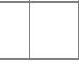
\includegraphics[max width=\textwidth]{2024_11_21_832f1bc2b626663f1df2g-11(3)}
 &  &  &  &  &  & 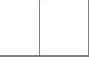
\includegraphics[max width=\textwidth]{2024_11_21_832f1bc2b626663f1df2g-11}
 & 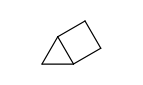
\includegraphics{smile-de37dda7c41172f87b8c1db2fe6e57f7b0c2332e} \\
\hline
\end{tabular}
\end{center}

\section*{Zadanie 29. (0-2 pkt)}
Rozwiąż równanie \(5 x\left(x^{3}+1\right)(2 x-8)\left(x^{2}+4\right)=0\)

\begin{center}
\begin{tabular}{|c|c|c|c|c|c|c|c|c|c|c|c|c|c|c|c|c|c|c|c|c|c|}
\hline
 &  &  &  &  &  &  &  &  &  &  &  &  & - &  & - & \textbackslash  &  &  & T & 到 &  \\
\hline
 &  &  &  &  &  &  &  &  &  &  &  &  &  &  &  &  &  &  &  &  &  \\
\hline
 &  &  &  &  &  &  &  &  &  &  &  &  &  &  &  &  &  &  &  &  &  \\
\hline
 &  &  &  &  &  &  &  &  &  &  &  &  &  &  &  &  &  &  &  &  &  \\
\hline
 &  &  &  &  &  &  &  &  &  &  &  &  &  &  &  &  &  &  &  &  &  \\
\hline
 &  &  &  &  &  &  &  &  &  &  &  &  &  &  &  &  &  &  &  &  &  \\
\hline
 &  &  &  &  &  &  &  &  &  &  &  &  &  &  &  &  &  &  &  &  &  \\
\hline
 &  &  &  &  &  &  &  &  &  &  &  &  &  &  &  &  &  &  &  &  &  \\
\hline
 &  &  &  &  &  &  &  &  &  &  &  &  &  &  &  &  &  &  &  &  &  \\
\hline
 &  &  &  &  &  &  &  &  &  &  &  &  &  &  &  &  &  &  &  &  &  \\
\hline
 &  &  &  &  &  &  &  &  &  &  &  &  &  &  &  &  &  &  &  &  &  \\
\hline
 &  &  &  &  &  &  &  &  &  &  &  &  &  &  &  &  &  &  &  &  &  \\
\hline
 &  &  &  &  &  &  &  &  &  &  &  &  &  &  &  &  &  &  &  &  &  \\
\hline
 &  &  &  &  &  &  &  &  &  &  &  &  &  &  &  &  &  &  &  &  &  \\
\hline
 &  &  &  &  &  &  &  &  &  &  &  &  &  &  &  &  &  &  &  &  &  \\
\hline
 &  &  &  &  &  &  &  &  &  &  &  &  &  &  &  &  &  &  &  &  &  \\
\hline
\end{tabular}
\end{center}

Odpowiedź:

\section*{Zadanie 30. (0-2 pkt)}
W dwóch pojemnikach znajdują się ponumerowane kule. W pierwszym pojemniku są kule z numerami: 1, 2, 3, 4, 5, w drugim z numerami: \(4,5,6,7,8,9\). Losujemy po jednej kuli z każdego pojemnika i tworzymy liczbę dwucyfrową. Numer kuli wylosowanej z pierwszego pojemnika jest cyfrą dziesiątek, numer kuli wylosowanej z drugiego pojemnika jest cyfrą jedności. Oblicz prawdopodobieństwo zdarzenia, że utworzona liczba jest podzielna przez 4.

\begin{center}
\begin{tabular}{|c|c|c|c|c|c|c|c|c|c|c|c|c|c|c|c|c|c|c|c|c|c|c|}
\hline
 &  &  &  &  &  &  &  &  &  &  &  &  &  &  &  &  &  &  &  &  &  &  \\
\hline
 &  &  &  &  &  &  &  &  &  &  &  &  &  &  &  &  &  &  &  &  &  &  \\
\hline
 &  &  &  &  &  &  &  &  &  &  &  &  &  &  &  &  &  &  &  &  &  &  \\
\hline
 &  &  &  &  &  &  &  &  &  &  &  &  &  &  &  &  &  &  &  &  &  &  \\
\hline
 &  &  &  &  &  &  &  &  &  &  &  &  &  &  &  &  &  &  &  &  &  &  \\
\hline
 &  &  &  &  &  &  &  &  &  &  &  &  &  &  &  &  &  &  &  &  &  &  \\
\hline
 &  &  &  &  &  &  &  &  &  &  &  &  &  &  &  &  &  &  &  &  &  &  \\
\hline
 &  &  &  &  &  &  &  &  &  &  &  &  &  &  &  &  &  &  &  &  &  &  \\
\hline
 &  &  &  &  &  &  &  &  &  &  &  &  &  &  &  &  &  &  &  &  &  &  \\
\hline
 &  &  &  &  &  &  &  &  &  &  &  &  &  &  &  &  &  &  &  &  &  &  \\
\hline
 &  &  &  &  &  &  &  &  &  &  &  &  &  &  &  &  &  &  &  &  &  &  \\
\hline
 &  &  &  &  &  &  &  &  &  &  &  &  &  &  &  &  &  &  &  &  &  &  \\
\hline
 &  &  &  &  &  &  &  &  &  &  &  &  &  &  &  &  &  &  &  &  &  &  \\
\hline
 &  &  &  &  &  &  &  &  &  &  &  &  &  &  &  &  &  &  &  &  &  &  \\
\hline
\end{tabular}
\end{center}

Odpowiedź:

\section*{Zadanie 31. (0-2 pkt)}
W trapezie prostokątnym \(A B C D\) (rysunek) punkt \(K\) jest punktem przecięcia wysokości \(D E\) i przekątnej \(A C\) tego trapezu. Wiedząc, że \(|C B|=|C D|=a \quad\) i \(\quad|A B|=b\) wykaż, że pole \(P\) czworokąta \(E B C K\) jest równe \(P=\frac{2 a^{2} b-a^{3}}{2 b}\).\\
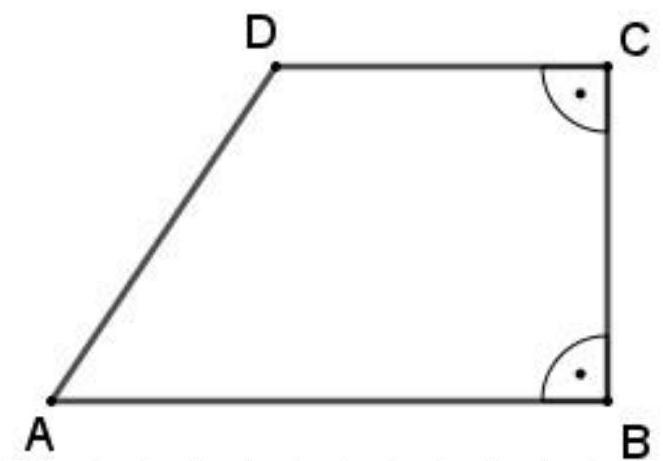
\includegraphics[max width=\textwidth, center]{2024_11_21_832f1bc2b626663f1df2g-13}\\

\includegraphics[max width=\textwidth, center]{2024_11_21_832f1bc2b626663f1df2g-13(1)}

Zadanie 32. (0 - 5 pkt)\\
Punkty \(A=\left(-\frac{1}{2} ;-1 \frac{1}{2}\right), B=\left(3 \frac{1}{2} ; \frac{1}{2}\right)\) są wierzchołkami trójkąta równoramiennego \(A B C\) o podstawie \(A B\). Ramię \(B C\) zawiera się w prostej o równaniu \(8 x+14 y-35=0\). Oblicz współrzędne punktu \(C\) i pole tego trójkąta.\\

\includegraphics[max width=\textwidth, center]{2024_11_21_832f1bc2b626663f1df2g-14}\\

\includegraphics[max width=\textwidth, center]{2024_11_21_832f1bc2b626663f1df2g-15}

\section*{Zadanie 33. (0 - 4 pkt)}
Funkcja kwadratowa \(y=f(x)\) przyjmuje wartości ujemne tylko dla \(x \in(-\infty,-2) \cup(5, \infty)\), a jej zbiorem wartości jest przedział \(\left(-\infty, \frac{49}{8}\right\rangle\). Zapisz wzór funkcji kwadratowej \(g(x)=f(x-2)\) w postaci ogólnej.\\

\includegraphics[max width=\textwidth, center]{2024_11_21_832f1bc2b626663f1df2g-16}

\section*{Zadanie 34. (0-4 pkt)}
Krawędź podstawy graniastosłupa prawidłowego czworokątnego ma długość 8 cm , a jego wysokość 12 cm . Połączono środki dwóch sąsiednich krawędzi dolnej podstawy oraz najbardziej odległy od tego odcinka wierzchołek górnej podstawy. Oblicz pole otrzymanego trójkąta.\\

\includegraphics[max width=\textwidth, center]{2024_11_21_832f1bc2b626663f1df2g-17}

Odpowiedź:

\section*{KOD}
\begin{center}
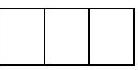
\includegraphics[max width=\textwidth]{2024_11_21_832f1bc2b626663f1df2g-18}
\end{center}

\section*{PESEL}
\begin{center}
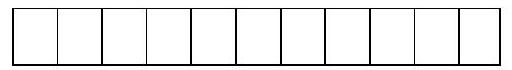
\includegraphics[max width=\textwidth]{2024_11_21_832f1bc2b626663f1df2g-18(1)}
\end{center}

WYPELNIA ZDAJĄCY

\begin{center}
\begin{tabular}{|c|c|c|c|c|}
\hline
\multirow{2}{*}{\(
\begin{gathered}
\mathrm{Nr} \\
\text { zad. }
\end{gathered}
\)} & \multicolumn{4}{|c|}{Odpowiedzi} \\
\hline
 & A & B & C & D \\
\hline
1 & ㅁ & - & - & - \\
\hline
2 & ㅁ & ㅁ & ㅁ & - \\
\hline
3 & ㅁ & ㅁ & ㅁ & - \\
\hline
4 & ㅁ & ㅁ & ㅁ & - \\
\hline
5 & ㅁ & ㅁ & ㅁ & - \\
\hline
6 & ㅁ & ㅁ & ㅁ & ㅁ \\
\hline
7 & ㅁ & ㅁ & ㅁ & ㅁ \\
\hline
8 & ㅁ & ㅁ & ㅁ & - \\
\hline
9 & ㅁ & ㅁ & ㅁ & - \\
\hline
10 & ㅁ & ㅁ & ㅁ & - \\
\hline
11 & ㅁ & ㅁ & ㅁ & - \\
\hline
12 & ㅁ & ㅁ & ㅁ & - \\
\hline
13 & ㅁ & ㅁ & ㅁ & - \\
\hline
14 & ㅁ & ㅁ & ㅁ & ㅁ \\
\hline
15 & ㅁ & ㅁ & ㅁ & - \\
\hline
16 & ㅁ & ㅁ & ㅁ & ㅁ \\
\hline
17 & ㅁ & ㅁ & ㅁ & ㅁ \\
\hline
18 & ㅁ & ㅁ & ㅁ & - \\
\hline
19 & ㅁ & ㅁ & ㅁ & - \\
\hline
20 & ㅁ & ㅁ & ㅁ & - \\
\hline
21 & ㅁ & ㅁ & ㅁ & ㅁ \\
\hline
22 & ㅁ & ㅁ & ㅁ & - \\
\hline
23 & ㅁ & ㅁ & ㅁ & - \\
\hline
24 & ㅁ & ㅁ & ㅁ & - \\
\hline
25 & ㅁ & ㅁ & ㅁ & - \\
\hline
\end{tabular}
\end{center}

WYPELNIA EGZAMINATOR

\begin{center}
\begin{tabular}{|c|c|c|c|c|c|c|}
\hline
Nr & \multicolumn{6}{|c|}{Punkty} \\
\hline
zad. & \(\mathbf{0}\) & \(\mathbf{1}\) & \(\mathbf{2}\) & \(\mathbf{3}\) & \(\mathbf{4}\) & \(\mathbf{5}\) \\
\hline
\(\mathbf{2 6}\) & \(\square\) & \(\square\) & \(\square\) &  &  &  \\
\hline
\(\mathbf{2 7}\) & \(\square\) & \(\square\) & \(\square\) &  &  &  \\
\hline
\(\mathbf{2 8}\) & \(\square\) & \(\square\) & \(\square\) &  &  &  \\
\hline
\(\mathbf{2 9}\) & \(\square\) & \(\square\) & \(\square\) &  &  &  \\
\hline
\(\mathbf{3 0}\) & \(\square\) & \(\square\) & \(\square\) &  &  &  \\
\hline
\(\mathbf{3 1}\) & \(\square\) & \(\square\) & \(\square\) &  &  &  \\
\hline
\(\mathbf{3 2}\) & \(\square\) & \(\square\) & \(\square\) & \(\square\) & \(\square\) & \(\square\) \\
\hline
\(\mathbf{3 3}\) & \(\square\) & \(\square\) & \(\square\) & \(\square\) & \(\square\) &  \\
\hline
\(\mathbf{3 4}\) & \(\square\) & \(\square\) & \(\square\) & \(\square\) & \(\square\) &  \\
\hline
\end{tabular}
\end{center}

SUMA PUNKTÓW


\end{document}